% Options for packages loaded elsewhere
\PassOptionsToPackage{unicode}{hyperref}
\PassOptionsToPackage{hyphens}{url}
%
\documentclass[
]{book}
\usepackage{amsmath,amssymb}
\usepackage{iftex}
\ifPDFTeX
  \usepackage[T1]{fontenc}
  \usepackage[utf8]{inputenc}
  \usepackage{textcomp} % provide euro and other symbols
\else % if luatex or xetex
  \usepackage{unicode-math} % this also loads fontspec
  \defaultfontfeatures{Scale=MatchLowercase}
  \defaultfontfeatures[\rmfamily]{Ligatures=TeX,Scale=1}
\fi
\usepackage{lmodern}
\ifPDFTeX\else
  % xetex/luatex font selection
\fi
% Use upquote if available, for straight quotes in verbatim environments
\IfFileExists{upquote.sty}{\usepackage{upquote}}{}
\IfFileExists{microtype.sty}{% use microtype if available
  \usepackage[]{microtype}
  \UseMicrotypeSet[protrusion]{basicmath} % disable protrusion for tt fonts
}{}
\makeatletter
\@ifundefined{KOMAClassName}{% if non-KOMA class
  \IfFileExists{parskip.sty}{%
    \usepackage{parskip}
  }{% else
    \setlength{\parindent}{0pt}
    \setlength{\parskip}{6pt plus 2pt minus 1pt}}
}{% if KOMA class
  \KOMAoptions{parskip=half}}
\makeatother
\usepackage{xcolor}
\usepackage{color}
\usepackage{fancyvrb}
\newcommand{\VerbBar}{|}
\newcommand{\VERB}{\Verb[commandchars=\\\{\}]}
\DefineVerbatimEnvironment{Highlighting}{Verbatim}{commandchars=\\\{\}}
% Add ',fontsize=\small' for more characters per line
\usepackage{framed}
\definecolor{shadecolor}{RGB}{248,248,248}
\newenvironment{Shaded}{\begin{snugshade}}{\end{snugshade}}
\newcommand{\AlertTok}[1]{\textcolor[rgb]{0.94,0.16,0.16}{#1}}
\newcommand{\AnnotationTok}[1]{\textcolor[rgb]{0.56,0.35,0.01}{\textbf{\textit{#1}}}}
\newcommand{\AttributeTok}[1]{\textcolor[rgb]{0.13,0.29,0.53}{#1}}
\newcommand{\BaseNTok}[1]{\textcolor[rgb]{0.00,0.00,0.81}{#1}}
\newcommand{\BuiltInTok}[1]{#1}
\newcommand{\CharTok}[1]{\textcolor[rgb]{0.31,0.60,0.02}{#1}}
\newcommand{\CommentTok}[1]{\textcolor[rgb]{0.56,0.35,0.01}{\textit{#1}}}
\newcommand{\CommentVarTok}[1]{\textcolor[rgb]{0.56,0.35,0.01}{\textbf{\textit{#1}}}}
\newcommand{\ConstantTok}[1]{\textcolor[rgb]{0.56,0.35,0.01}{#1}}
\newcommand{\ControlFlowTok}[1]{\textcolor[rgb]{0.13,0.29,0.53}{\textbf{#1}}}
\newcommand{\DataTypeTok}[1]{\textcolor[rgb]{0.13,0.29,0.53}{#1}}
\newcommand{\DecValTok}[1]{\textcolor[rgb]{0.00,0.00,0.81}{#1}}
\newcommand{\DocumentationTok}[1]{\textcolor[rgb]{0.56,0.35,0.01}{\textbf{\textit{#1}}}}
\newcommand{\ErrorTok}[1]{\textcolor[rgb]{0.64,0.00,0.00}{\textbf{#1}}}
\newcommand{\ExtensionTok}[1]{#1}
\newcommand{\FloatTok}[1]{\textcolor[rgb]{0.00,0.00,0.81}{#1}}
\newcommand{\FunctionTok}[1]{\textcolor[rgb]{0.13,0.29,0.53}{\textbf{#1}}}
\newcommand{\ImportTok}[1]{#1}
\newcommand{\InformationTok}[1]{\textcolor[rgb]{0.56,0.35,0.01}{\textbf{\textit{#1}}}}
\newcommand{\KeywordTok}[1]{\textcolor[rgb]{0.13,0.29,0.53}{\textbf{#1}}}
\newcommand{\NormalTok}[1]{#1}
\newcommand{\OperatorTok}[1]{\textcolor[rgb]{0.81,0.36,0.00}{\textbf{#1}}}
\newcommand{\OtherTok}[1]{\textcolor[rgb]{0.56,0.35,0.01}{#1}}
\newcommand{\PreprocessorTok}[1]{\textcolor[rgb]{0.56,0.35,0.01}{\textit{#1}}}
\newcommand{\RegionMarkerTok}[1]{#1}
\newcommand{\SpecialCharTok}[1]{\textcolor[rgb]{0.81,0.36,0.00}{\textbf{#1}}}
\newcommand{\SpecialStringTok}[1]{\textcolor[rgb]{0.31,0.60,0.02}{#1}}
\newcommand{\StringTok}[1]{\textcolor[rgb]{0.31,0.60,0.02}{#1}}
\newcommand{\VariableTok}[1]{\textcolor[rgb]{0.00,0.00,0.00}{#1}}
\newcommand{\VerbatimStringTok}[1]{\textcolor[rgb]{0.31,0.60,0.02}{#1}}
\newcommand{\WarningTok}[1]{\textcolor[rgb]{0.56,0.35,0.01}{\textbf{\textit{#1}}}}
\usepackage{longtable,booktabs,array}
\usepackage{calc} % for calculating minipage widths
% Correct order of tables after \paragraph or \subparagraph
\usepackage{etoolbox}
\makeatletter
\patchcmd\longtable{\par}{\if@noskipsec\mbox{}\fi\par}{}{}
\makeatother
% Allow footnotes in longtable head/foot
\IfFileExists{footnotehyper.sty}{\usepackage{footnotehyper}}{\usepackage{footnote}}
\makesavenoteenv{longtable}
\usepackage{graphicx}
\makeatletter
\def\maxwidth{\ifdim\Gin@nat@width>\linewidth\linewidth\else\Gin@nat@width\fi}
\def\maxheight{\ifdim\Gin@nat@height>\textheight\textheight\else\Gin@nat@height\fi}
\makeatother
% Scale images if necessary, so that they will not overflow the page
% margins by default, and it is still possible to overwrite the defaults
% using explicit options in \includegraphics[width, height, ...]{}
\setkeys{Gin}{width=\maxwidth,height=\maxheight,keepaspectratio}
% Set default figure placement to htbp
\makeatletter
\def\fps@figure{htbp}
\makeatother
\setlength{\emergencystretch}{3em} % prevent overfull lines
\providecommand{\tightlist}{%
  \setlength{\itemsep}{0pt}\setlength{\parskip}{0pt}}
\setcounter{secnumdepth}{5}
\usepackage{booktabs}
\ifLuaTeX
  \usepackage{selnolig}  % disable illegal ligatures
\fi
\usepackage[]{natbib}
\bibliographystyle{plainnat}
\IfFileExists{bookmark.sty}{\usepackage{bookmark}}{\usepackage{hyperref}}
\IfFileExists{xurl.sty}{\usepackage{xurl}}{} % add URL line breaks if available
\urlstyle{same}
\hypersetup{
  pdftitle={Theory-driven analysis of ecological data: a practical handbook},
  pdfauthor={us},
  hidelinks,
  pdfcreator={LaTeX via pandoc}}

\title{Theory-driven analysis of ecological data: a practical handbook}
\author{us}
\date{2024-01-08}

\usepackage{amsthm}
\newtheorem{theorem}{Theorem}[chapter]
\newtheorem{lemma}{Lemma}[chapter]
\newtheorem{corollary}{Corollary}[chapter]
\newtheorem{proposition}{Proposition}[chapter]
\newtheorem{conjecture}{Conjecture}[chapter]
\theoremstyle{definition}
\newtheorem{definition}{Definition}[chapter]
\theoremstyle{definition}
\newtheorem{example}{Example}[chapter]
\theoremstyle{definition}
\newtheorem{exercise}{Exercise}[chapter]
\theoremstyle{definition}
\newtheorem{hypothesis}{Hypothesis}[chapter]
\theoremstyle{remark}
\newtheorem*{remark}{Remark}
\newtheorem*{solution}{Solution}
\begin{document}
\maketitle

{
\setcounter{tocdepth}{1}
\tableofcontents
}
\chapter{About Bookdown}\label{about-bookdown}

This is a \emph{sample} book written in \textbf{Markdown}. You can use anything that Pandoc's Markdown supports; for example, a math equation \(a^2 + b^2 = c^2\).

\section{Usage}\label{usage}

Each \textbf{bookdown} chapter is an .Rmd file, and each .Rmd file can contain one (and only one) chapter. A chapter \emph{must} start with a first-level heading: \texttt{\#\ A\ good\ chapter}, and can contain one (and only one) first-level heading.

Use second-level and higher headings within chapters like: \texttt{\#\#\ A\ short\ section} or \texttt{\#\#\#\ An\ even\ shorter\ section}.

The \texttt{index.Rmd} file is required, and is also your first book chapter. It will be the homepage when you render the book.

\section{Render book}\label{render-book}

You can render the HTML version of this example book without changing anything:

\begin{enumerate}
\def\labelenumi{\arabic{enumi}.}
\item
  Find the \textbf{Build} pane in the RStudio IDE, and
\item
  Click on \textbf{Build Book}, then select your output format, or select ``All formats'' if you'd like to use multiple formats from the same book source files.
\end{enumerate}

Or build the book from the R console:

\begin{Shaded}
\begin{Highlighting}[]
\NormalTok{bookdown}\SpecialCharTok{::}\FunctionTok{render\_book}\NormalTok{()}
\end{Highlighting}
\end{Shaded}

To render this example to PDF as a \texttt{bookdown::pdf\_book}, you'll need to install XeLaTeX. You are recommended to install TinyTeX (which includes XeLaTeX): \url{https://yihui.org/tinytex/}.

\section{Preview book}\label{preview-book}

As you work, you may start a local server to live preview this HTML book. This preview will update as you edit the book when you save individual .Rmd files. You can start the server in a work session by using the RStudio add-in ``Preview book'', or from the R console:

\begin{Shaded}
\begin{Highlighting}[]
\NormalTok{bookdown}\SpecialCharTok{::}\FunctionTok{serve\_book}\NormalTok{()}
\end{Highlighting}
\end{Shaded}

\section{Here are some useful things for writing the book using bookdown}\label{here-are-some-useful-things-for-writing-the-book-using-bookdown}

All chapters start with a first-level heading followed by your chapter title, like the line above. There should be only one first-level heading (\texttt{\#}) per .Rmd file.

\subsection{A section}\label{a-section}

All chapter sections start with a second-level (\texttt{\#\#}) or higher heading followed by your section title, like the sections above and below here. You can have as many as you want within a chapter.

\subsubsection*{An unnumbered section}\label{an-unnumbered-section}
\addcontentsline{toc}{subsubsection}{An unnumbered section}

Chapters and sections are numbered by default. To un-number a heading, add a \texttt{\{.unnumbered\}} or the shorter \texttt{\{-\}} at the end of the heading, like in this section.

\section{Cross-references}\label{cross}

Cross-references make it easier for your readers to find and link to elements in your book.

\subsection{Chapters and sub-chapters}\label{chapters-and-sub-chapters}

There are two steps to cross-reference any heading:

\begin{enumerate}
\def\labelenumi{\arabic{enumi}.}
\tightlist
\item
  Label the heading: \texttt{\#\ Hello\ world\ \{\#nice-label\}}.

  \begin{itemize}
  \tightlist
  \item
    Leave the label off if you like the automated heading generated based on your heading title: for example, \texttt{\#\ Hello\ world} = \texttt{\#\ Hello\ world\ \{\#hello-world\}}.
  \item
    To label an un-numbered heading, use: \texttt{\#\ Hello\ world\ \{-\#nice-label\}} or \texttt{\{\#\ Hello\ world\ .unnumbered\}}.
  \end{itemize}
\item
  Next, reference the labeled heading anywhere in the text using \texttt{\textbackslash{}@ref(nice-label)}; for example, please see Chapter \ref{cross}.

  \begin{itemize}
  \tightlist
  \item
    If you prefer text as the link instead of a numbered reference use: \hyperref[cross]{any text you want can go here}.
  \end{itemize}
\end{enumerate}

\subsection{Captioned figures and tables}\label{captioned-figures-and-tables}

Figures and tables \emph{with captions} can also be cross-referenced from elsewhere in your book using \texttt{\textbackslash{}@ref(fig:chunk-label)} and \texttt{\textbackslash{}@ref(tab:chunk-label)}, respectively.

See Figure \ref{fig:nice-fig}.

\begin{Shaded}
\begin{Highlighting}[]
\FunctionTok{par}\NormalTok{(}\AttributeTok{mar =} \FunctionTok{c}\NormalTok{(}\DecValTok{4}\NormalTok{, }\DecValTok{4}\NormalTok{, .}\DecValTok{1}\NormalTok{, .}\DecValTok{1}\NormalTok{))}
\FunctionTok{plot}\NormalTok{(pressure, }\AttributeTok{type =} \StringTok{\textquotesingle{}b\textquotesingle{}}\NormalTok{, }\AttributeTok{pch =} \DecValTok{19}\NormalTok{)}
\end{Highlighting}
\end{Shaded}

\begin{figure}

{\centering 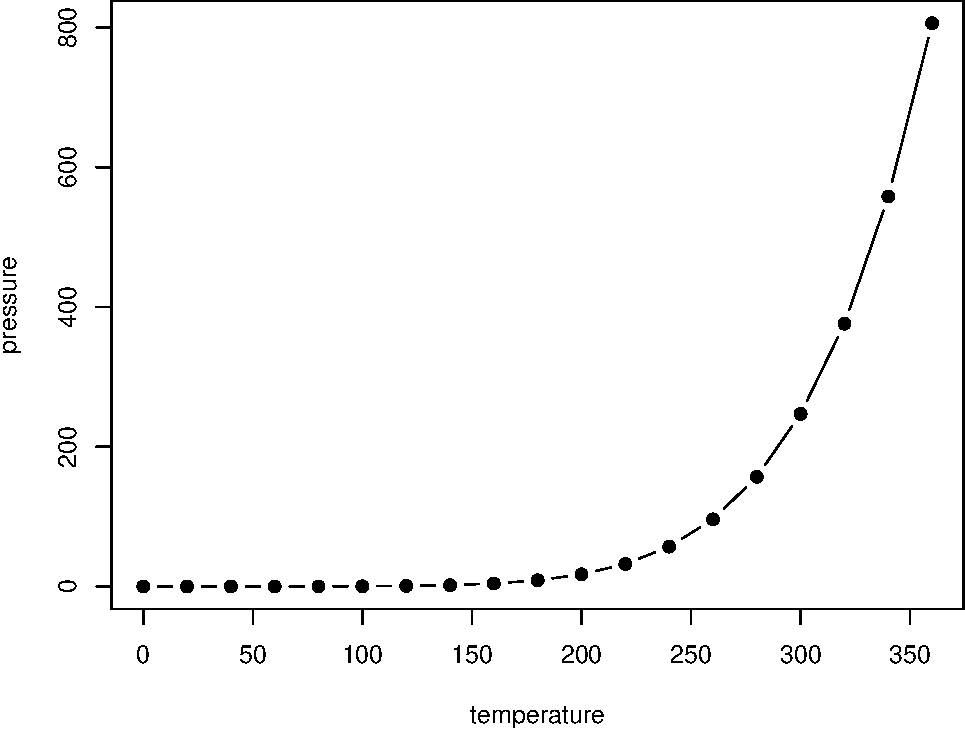
\includegraphics[width=0.8\linewidth]{_main_files/figure-latex/nice-fig-1} 

}

\caption{Here is a nice figure!}\label{fig:nice-fig}
\end{figure}

Don't miss Table \ref{tab:nice-tab}.

\begin{Shaded}
\begin{Highlighting}[]
\NormalTok{knitr}\SpecialCharTok{::}\FunctionTok{kable}\NormalTok{(}
  \FunctionTok{head}\NormalTok{(pressure, }\DecValTok{10}\NormalTok{), }\AttributeTok{caption =} \StringTok{\textquotesingle{}Here is a nice table!\textquotesingle{}}\NormalTok{,}
  \AttributeTok{booktabs =} \ConstantTok{TRUE}
\NormalTok{)}
\end{Highlighting}
\end{Shaded}

\begin{table}

\caption{\label{tab:nice-tab}Here is a nice table!}
\centering
\begin{tabular}[t]{rr}
\toprule
temperature & pressure\\
\midrule
0 & 0.0002\\
20 & 0.0012\\
40 & 0.0060\\
60 & 0.0300\\
80 & 0.0900\\
\addlinespace
100 & 0.2700\\
120 & 0.7500\\
140 & 1.8500\\
160 & 4.2000\\
180 & 8.8000\\
\bottomrule
\end{tabular}
\end{table}

\section{Parts}\label{parts}

You can add parts to organize one or more book chapters together. Parts can be inserted at the top of an .Rmd file, before the first-level chapter heading in that same file.

Add a numbered part: \texttt{\#\ (PART)\ Act\ one\ \{-\}} (followed by \texttt{\#\ A\ chapter})

Add an unnumbered part: \texttt{\#\ (PART\textbackslash{}*)\ Act\ one\ \{-\}} (followed by \texttt{\#\ A\ chapter})

Add an appendix as a special kind of un-numbered part: \texttt{\#\ (APPENDIX)\ Other\ stuff\ \{-\}} (followed by \texttt{\#\ A\ chapter}). Chapters in an appendix are prepended with letters instead of numbers.

\section{Footnotes and citations}\label{footnotes-and-citations}

\subsection{Footnotes}\label{footnotes}

Footnotes are put inside the square brackets after a caret \texttt{\^{}{[}{]}}. Like this one \footnote{This is a footnote.}.

\subsection{Citations}\label{citations}

Reference items in your bibliography file(s) using \texttt{@key}.

For example, we are using the \textbf{bookdown} package \citep{R-bookdown} (check out the last code chunk in index.Rmd to see how this citation key was added) in this sample book, which was built on top of R Markdown and \textbf{knitr} \citep{xie2015} (this citation was added manually in an external file book.bib).
Note that the \texttt{.bib} files need to be listed in the index.Rmd with the YAML \texttt{bibliography} key.

The RStudio Visual Markdown Editor can also make it easier to insert citations: \url{https://rstudio.github.io/visual-markdown-editing/\#/citations}

\section{Blocks}\label{blocks}

\subsection{Equations}\label{equations}

Here is an equation.

\begin{equation} 
  f\left(k\right) = \binom{n}{k} p^k\left(1-p\right)^{n-k}
  \label{eq:binom}
\end{equation}

You may refer to using \texttt{\textbackslash{}@ref(eq:binom)}, like see Equation \eqref{eq:binom}.

\subsection{Theorems and proofs}\label{theorems-and-proofs}

Labeled theorems can be referenced in text using \texttt{\textbackslash{}@ref(thm:tri)}, for example, check out this smart theorem \ref{thm:tri}.

\begin{theorem}
\protect\hypertarget{thm:tri}{}\label{thm:tri}For a right triangle, if \(c\) denotes the \emph{length} of the hypotenuse
and \(a\) and \(b\) denote the lengths of the \textbf{other} two sides, we have
\[a^2 + b^2 = c^2\]
\end{theorem}

Read more here \url{https://bookdown.org/yihui/bookdown/markdown-extensions-by-bookdown.html}.

\subsection{Callout blocks}\label{callout-blocks}

The R Markdown Cookbook provides more help on how to use custom blocks to design your own callouts: \url{https://bookdown.org/yihui/rmarkdown-cookbook/custom-blocks.html}

\section{Sharing your book}\label{sharing-your-book}

\subsection{Publishing}\label{publishing}

HTML books can be published online, see: \url{https://bookdown.org/yihui/bookdown/publishing.html}

\subsection{404 pages}\label{pages}

By default, users will be directed to a 404 page if they try to access a webpage that cannot be found. If you'd like to customize your 404 page instead of using the default, you may add either a \texttt{\_404.Rmd} or \texttt{\_404.md} file to your project root and use code and/or Markdown syntax.

\subsection{Metadata for sharing}\label{metadata-for-sharing}

Bookdown HTML books will provide HTML metadata for social sharing on platforms like Twitter, Facebook, and LinkedIn, using information you provide in the \texttt{index.Rmd} YAML. To setup, set the \texttt{url} for your book and the path to your \texttt{cover-image} file. Your book's \texttt{title} and \texttt{description} are also used.

This \texttt{gitbook} uses the same social sharing data across all chapters in your book- all links shared will look the same.

Specify your book's source repository on GitHub using the \texttt{edit} key under the configuration options in the \texttt{\_output.yml} file, which allows users to suggest an edit by linking to a chapter's source file.

Read more about the features of this output format here:

\url{https://pkgs.rstudio.com/bookdown/reference/gitbook.html}

Or use:

\begin{Shaded}
\begin{Highlighting}[]
\NormalTok{?bookdown}\SpecialCharTok{::}\NormalTok{gitbook}
\end{Highlighting}
\end{Shaded}

\chapter{Preambule}\label{preambule}

Who is the textbook for?

\chapter{Why mathematical models? (old title: Background)}\label{why-mathematical-models-old-title-background}

\section{The scientific method}\label{the-scientific-method}

Why do we need model in ecology? Before answering that question, let's first step back and reflect on the process by which science is carried out. The scientific method is an empirical method for acquiring knowledge that has characterized the development of science since at least the 17th century.

Science (through the scientific method) can build on previous knowledge and develop a more sophisticated understanding of its topics of study over time.

\begin{itemize}
\item
  It involves careful observation/ Formulation of a question
\item
  Hypothesis: A hypothesis is a conjecture (hypothetical explanations), based on the observation/the knowledge obtained while formulating the question, that may explain any given behavior. A scientific hypothesis must be falsifiable, implying that it is possible to identify a possible outcome of an experiment or observation that conflicts with predictions deduced from the hypothesis; otherwise, the hypothesis cannot be meaningfully tested.
  Falsifiability is a deductive standard of evaluation of scientific theories and hypotheses, introduced by the philosopher of science Karl Popper in his book The Logic of Scientific Discovery (1934).{[}B{]} A theory or hypothesis is falsifiable (or refutable) if it can be logically contradicted by an empirical test.
\item
  Prediction: The prediction step deduces the logical consequences of the hypothesis before the outcome is known.
\item
  Testing: Hypotheses are tested by conducting experiments or gathering observations. The purpose of the test is to determine whether observations agree with or conflict with the expectations deduced from a hypothesis.
\item
  Next action to take: refinement (or elimination) of the hypotheses based on the experimental findings.
\end{itemize}

Although procedures vary from one field of inquiry to another, the underlying process is frequently the same. In sum, the process is as follows making conjectures (hypotheses), deriving predictions from them as logical consequences, and then carrying out experiments based on those predictions to determine whether the original conjecture was correct.

The scientific method is an iterative, cyclical process through which information is continually revised

\section{A feedback loop involving data and models}\label{a-feedback-loop-involving-data-and-models}

A scientific understanding of the biological world arises when ideas about how nature works are formalized, tested, refined, and then tested again.

Scientific inquiry should operate as a feedback loop in which theory that describes the natural world is developed, tested empirically through carefully articulated hypotheses, modified to better represent reality, and then tested again.

When this feedback loop works, theory provides a framework to guide inquiry, experimental design, and the interpretation of observed patterns, supplies mathematical tools to harness information from collected data, and connects individual experiments to general ideas about how nature operates.

In turn, empirical research can be used to support, refute, or revise theoretical predictions, indicate which theoretical assumptions are consistent with the natural world, and point theoreticians to overlooked processes that can be integrated into models.

\textbf{But: there is a disconnect between theoretical and empirical research}

Although the benefits of feedback between theoretical and empirical research are widely acknowledged by ecologists, this link is still not as strong as it could be in ecological research.

Disconnect between empirical and theoretical work in ecology (Lomnicki 1988; Kareiva 1989; Fawcett and Higginson 2012; Scheiner 2013; Haller 2014; Rossberg et al.~2019).

Up to 45\% of articles on empirical ecology make no mention of any theory whatsoever (Scheiner 2013), and fewer than 10\% of ecologists and evolutionary biologists agree with the statement that `theoretical findings drive empirical work' in their fields (Haller 2014).

\textbf{Why this disconnection?}

\begin{itemize}
\tightlist
\item
  A lack of theoretical training in ecology (Rossberg et al.~2019).
\item
  A lack of motivation on the part of some theoreticians to engage with the language of empiricists (Grimm 1994) or with the elements of nature that empiricists focus on (Krebs 1988).
\item
  A general lack of mutual appreciation between empiricists and theoreticians (Haller 2014).
\item
  Persistent communication barriers between these two groups (Servedio 2020), in particular that theory is expressed in the langage of math (some ecologists may not have formal background in math and theoretical papers may not be written with a general audience, not always explaining asumptions, terminology and notations), some aspects of the theory may seem inaccessible by some, the more equations an ecology and evolutionary biology article contains, the fewer citations it receives (Fawcett and Higginson 2012).
\end{itemize}

This barrier presents a major challenge to the full integration of theoretical and empirical work in ecology.

\textbf{A better integration of theory into empirical work is needed} (Caswell 1988; Pickett et al.~2010; Marquet et al.~2014; Servedio et al.~2014; Servedio 2020).

This is especially important in the context of global change.

\section{How and why are mathematical models created?}\label{how-and-why-are-mathematical-models-created}

\subsection{What is theory?}\label{what-is-theory}

We define ecological theory broadly as an explanation of an ecological phenomenon. These explanations take the form of narratives that explain how an ecological process works or why an ecological pattern is observed and that become scientifically useful when expressed in a logical structure (Pickett et al.~2010; Rossberg et al.~2019).

Maris et al.~2017: Scientific theories contain universal or general propositions regarding the system in question; they generally encompass a set of models, or rules to build models, as representations of the properties and dynamics of target systems. Models can then be expressed as hypotheses within a formal framework (van Fraassen 1980, Giere 2004).

The transformation of an idea in narrative form into a logical, testable theory often, though not always, involves the use of models (Otto and Rosales 2020).

\subsection{What's a model?}\label{whats-a-model}

\url{https://en.wikipedia.org/wiki/Ecosystem_model}
If I say the word ``model'' what comes to your mind (everything, even not related to science)? (write on board) Models (Claudia Schiffer), miniatures, maps, mathematical models\ldots. What are the common elements?

The concept of a model is derived from scale models, referring to simplified replicas of larger structures such as, for instance, buildings or ships. This implies a structural similarity between a model and its original.
Thus, models are simplified representations of certain aspects of our study systems.
Models are idealized and simplified versions of reality, just as architectural models represent key features of complex structures and model organisms represent a group of organisms that share common attributes (Kokko 2007).
Models can be as simple as a verbal statement about a subject or two boxes connected by an arrow to represent some relationship. Alternatively, models can be extremely complex and detailed, such as a mathematical description of the pathways of nitrogen transformations within ecosystems.

Models can be conceptual (e.g.~diagram of boxes and arrows; boxes = state variables, arrows = relationships) or quantitative.

A mathematical model is an equation or a set of equations that describes how different aspects of a system relate to one another (Otto and Day 2007). (a set of mathematical expressions)

They can be phenomenological or mechanistic (Grainger et al.~2022).

Theory and math are not inexorably linked. Indeed, many excellent theories do not involve math (e.g., the theory of evolution by natural selection; Darwin 1859), and many uses of math in ecology are not theory (e.g., practical applications of statistics).

intro Kokko's book
models are an idealized, simplified version of the real world; e.g.~maps
Therefore they are not real. They're incomplete, they're wrong.
``all models are false but some models are useful''
\url{https://en.wikipedia.org/wiki/All_models_are_wrong}

The systems we're interested in are complex. How can we hope capturing the complexity of reality? We can't.
And if we did it would not be helpful (if models are as complex as reality).
e.g.~map
- too many parameters to measure (would require too much time and resources)
- the equations are insoluble and require too long to run on even a good computer
- even if soluble, we might not be able to understand the results

Modeling involves a choice what to include and what to leave out.
We need to simplify systems in a way that preserves the essential features of the system (depending on our interest).  this means that our big task as modelers is to decide what goes in the model and what doesn't. The art of modeling is to decide which aspect of reality one can sacrifice and which ones are crucial to retain.

The tension between realism, generality, and precision:
Levins 1966
\url{https://v4.chriskrycho.com/2016/realism-generality-and-precision-in-tension.html}

We want to work with manageable models which max generality, realism and precision towards the goals of understanding and predicting\ldots. But this cannot be done.

One can sacrifice generality to realism and precision. E.g. fisheries; good measurement of shot-time behavior, numerical solution  precise testable predictions applicable to a particular situation).

One can sacrifice realism to generality and precision. E.g. physics-like models (general equations such as LV) -\textgreater{} the way in which nature deviates from theory will indicate where further complexity will be useful.

One can sacrifice precision to realism and generality. E.g. MacArthur 1965. People concerned with the qualitative behavior (not quantitative). Graphical models.

Note that the choice made on what to sacrifice might depend on the stage of a research program:
At the conceptual stage of research models are used to further develop
theory. Models allow to do thoughts experiments. `All else being equal' what
is the effect of a certain factor or process? Conceptual models are thinking aids rather than investigations of real phenomena.
At the other extreme lies the practical stage, where models are used to closely
examine real-life phenomena. At the practical stage models are used for purposes such as inference from empirical data, making quantitative predictions concerning future system dynamics, or effects of studied factors, and guiding management decisions. These models comprise `statistical' models, `computer models', etc. Their aim is to make accurate statements about the studied system given the circumstances in the real world.

\subsection{Why modeling? Model -- theory}\label{why-modeling-model-theory}

Models do not investigate nature. Instead, they investigate the validity of our own thinking. Models are `thinking aids'. They exist because we need them to help us explore things: none of us was born with a supercomputer. P. 8 Kokko. The most important function of models is to order our thoughts. With models we formulate what we (think we) know about the world, and we may use them to perform thought experiments through `what if' scenarios. Modèle = experimentation pour poser des questions.
 models allow to explore ideas that might not be doable experimentally or for financial reasons.

Another important use of models is to function as an idealization of the world. Models
force us to make a choice concerning which aspects of `the real world' we include into
our description and which we choose to ignore (for the moment). This is true for verbal
as well as mathematical models. Mathematical formulations reveal implicit
assumptions and thus force us to be explicit. The translation of ideas in a theoretician' s mind into math on a page serves several purposes:
- math provides a clearer and more objective expression of relationships,
- it brings to light assumptions and logical errors that may be obscured in verbal hypotheses,
- and it places ideas and hypotheses into a concrete and concise form (Grimm 1994; Kokko 2007; Marquet et al.~2014; Otto and Rosales 2020).

Primer of eco with R p.~5:
The role of theory is 3 fold:
We like theory to allow us to describe the pattern in sufficient detail to
Provide a mecha explanation for how the plants grew as fast or slowly as it did
Allow us to make predictions about the pop size in the future
Allow us to generalize about other pop or sp
These goals typically compete with each other so real models are mathematical descriptions that result from tradeoffs among these goals which depend on our needs (cf Levins 1966).

Cf Virginie Maris -- predictive ecology
Article fundamental ecology is fundamental

We propose that two types of prediction should be distinguished:
- corroboratory-prediction is linked to the validation of theories; it refers to a step in the scientific process of understanding: hypotheses, models/theory are tested by comparing what is expected to occur (i.e.~predicted) with what actually occurs. It is a tense-neutral tool used to corroborate scientific hypotheses.
- and anticipatory-prediction is linked to the description of possible futures we seek to anticipate possible futures. It builds anticipations of the future under the assumption of some hypotheses being valid.

Note that anticipatory predictions are more and more expected in the context of global change (society's demand). Some people argue that with big data, we don't need theories anymore but we can use computing and stat tools to predict (although some people remain skeptical).

\subsection{The ingredients of models: How Is Mathematical Theory Created?}\label{the-ingredients-of-models-how-is-mathematical-theory-created}

The process of expressing theory in mathematical terms can seem mysterious to some. Here are the typical steps that a theoretician takes when creating a mathematical model (Otto and Day 2007; Bolker 2008):

\textbf{Step 1: The Motivation}

The first step in theory creation often parallels that of empirical research: the theoretician thinks of a biological question that she is interested in or a biological process that she wants to understand. The question may be motivated by
- an unsolved problem, for example, how temperature affects consumer-resource dynamics (O'Connor et al.~2011; DeLong and Lyon 2020).
- Or it could be motivated by an empirical observation, for example, evidence of interspecific differences in plant species' susceptibility to pathogens and an interest in the implications for plant coexistence (Stump and Comita 2018; Ke and Wan 2020).
- Or it may be motivated by a practical problem, for example, the need to understand how population structure influences COVID-19 dynamics (Britton et al.~2020).
- the creation of new theory is motivated by the desire to extend an existing model rather than to develop a new model from scratch. Indeed, most models are variants of previous models, extended to include different biological features, to tailor the model to a new system, or to address a slightly different question.
- One underappreciated initial goal of some theory is to provide a proof of concept that verifies or refutes ideas that may have previously been expressed only verbally (Servedio 2020). This use of theory demonstrates that something can happen under certain conditions but not necessarily that it is likely to occur under all or even most conditions (Servedio et al.~2014; Otto and Rosales 2020; Servedio 2020). These models can serve as hypothesis tests themselves and may not be meant to be tested empirically (Caswell 1988; Servedio et al.~2014).

\textbf{Step 2: The Method}

Next, the theoretician looks at the approaches that theory addressing similar questions has used and decides whether these approaches are relevant, justified, and suitable. The approach a theoretician takes is likely to be guided and constrained by her background; for example, a theoretician who is most familiar with dynamical models (those that track how a system changes over time) may be drawn to research questions that can be answered by that type of model, just as an empiricist who works with plankton mesocosms may focus on questions that are well suited to that approach.
New model builds on, tweaks, and combines existing models compared with conceiving of an entirely new mathematical approach.

\textbf{Step 3: The Equations}

In this step, the theoretician first decides which parameters and variables are necessary to describe the biological process of interest. A parameter is a quantity that has a value that does not vary within a given equation (e.g., resource supply rate), while a variable is a quantity whose value can vary within the equation, for example, through time (e.g., population size). In the simple model describing a linear relationship between x and y ( y p mx 1 b), x and y are variables (there are multiple values of x and y), and m (the slope) and b (the y-intercept) are parameters (there is only one slope and one y-intercept for this equation). Note that while parameters do not vary within an equation, the biological processes that they represent do vary in nature (e.g., across space, time, organism identity), and changing the value of parameters and exploring how that affects outcomes of interest is a common exercise in theory development (see ``numerical approaches'' below). A helpful exercise when deciding how multiple related equations should be written out is to draw stock and flow diagrams that show the relationship between the different variables in each equation (Otto and Day 2007).

In determining the equations, the theoretician must make difficult choices between how broadly the model can be applied across systems (generality), how closely the model mimics real-world processes (realism), and whether the model produces specific quantitative predictions or general qualitative predictions (precision) (Levins 1966; Servedio et al.~2014; Bodner et al.~2020). For example, models can be written with more terms or relationships to capture more biological detail, but additional terms may render the model less general. Note that the aim of mathematical models is to increase our understanding of some phenomenon, not to describe nature perfectly, and so a model making unrealistic assumptions or simplifying a process is not necessarily a failing of the theory or a reason to discount its ability to guide empirical research (Levins 1966; Pielou 1969; Grimm 1994; Kokko 2007; Phillips 2015; Servedio 2020). Just as empirical studies vary widely in their realism, from field-based observational studies to highly manipulated lab experiments, so, too, do ecological models. And just as each type of empirical study has value, so, too, does each type of theory.

The ingredients
The variables
The parameters
The processes involved
Choice of scale
Hypothesis of what to include/exclude
The technical choices (time discrete/continuous, space or not, discrete or continuous\ldots.)

What's the optimal complexity of a model?
It depends on the question. Give example: map.

A model should include all the relevant details for the particular question at hand, but it should be kept so simple that it can be understood.

\textbf{Step 4: The Analysis}

The theoretician then uses mathematical procedures to understand the behavior of her equations within the range of parameters that she is interested in exploring This can include solving for equilibria, investigating the stability of the equilibria, or studying how a response of interest (e.g., equilibrium density) varies across a range of parameters. These are common ways of determining the outcome of the processes being modeled.

Models can be analyzed analytically or numerically. Analytical approaches use mathematical techniques to solve the equation (i.e., find the equation that has the output of interest on the left-hand side) (table S1, available online). This approach requires mathematical labor but produces more general conclusions (Otto andDay 2007). Numerical approaches (e.g., simulations) involve setting model parameters to specific values and observing the outcome graphically or as numeric values (table S1). Here, conclusions are limited to the specific range of parameter values being explored, but because no analytical solutions are needed, theoreticians may turn to this approach when a model is too complex to be approached analytically. Numerical approaches are somewhat akin to empirical experiments in that the theoretician varies a specific process (e.g., resource supply rate) to determine how that affects an ecological outcome (e.g., consumer population density). While analyzing a model' s behavior cannot match the biological realism of an empirical experiment, it does allow researchers to hold potentially confounding factors constant and to explore a wide range of parameter space, whereas empirical experiments need to randomize factors that cannot be controlled (e.g., individuals, sites) and are often logistically constrained to smaller ranges or discrete categories (e.g., low vs.~high). Likewise, the ability to depart from the realities and constraints of the natural world allows theoreticians to explore questions that would be difficult or impossible to address empirically, such as the consequences of very long timescales, complex interactions, or extreme trait values.

It's important to note that theory can have a major influence on a field without any empirical testing, for example, theory demonstrating that transient dynamics can be prevalent and long lasting (Hastings 2001). Recognizing that not all theory was necessarily meant to be tested empirically can help empiricists focus on the types of theory that are most relevant to their scientific goals.

\section{Modelling in ecology}\label{modelling-in-ecology}

\subsection{A quick history}\label{a-quick-history}

\subsection{Specificities of ecology}\label{specificities-of-ecology}

Variability + time*space + local interactions + observations through both experiments and field studies + open systems
Formalisation,simplifications often used in ecology, assumptions, \ldots{}

\subsection{Ecological data, uncertainties, sampling}\label{ecological-data-uncertainties-sampling}

At different organisational scales: individual, population, community, ecosystem and all meta-

\subsection{Mathematical modelling / computational approaches (lots to discuss here from Game of life type stuff/von Neumann to IBMs/ABMs note: Grimm is not universally representative ;-) ) ?}\label{mathematical-modelling-computational-approaches-lots-to-discuss-here-from-game-of-life-type-stuffvon-neumann-to-ibmsabms-note-grimm-is-not-universally-representative--}

\section{Appendices}\label{appendices}

\subsection{Appendices: Primer on vectors and matrices (multidimensional data)}\label{appendices-primer-on-vectors-and-matrices-multidimensional-data}

\subsection{Appendices: Primer on analysis, dérivées, Taylor series, minimum/maximum\ldots{}}\label{appendices-primer-on-analysis-duxe9rivuxe9es-taylor-series-minimummaximum}

\subsection{Appendices: Removing dimensions, dimensional analysis}\label{appendices-removing-dimensions-dimensional-analysis}

\chapter{Mathematical (or ``process-based''?) modeling}\label{mathematical-or-process-based-modeling}

Intro pour expliquer la logique de l'agencement des chapitres

\section{Finite numbers of individuals (stochastic models)}\label{finite-numbers-of-individuals-stochastic-models}

\subsection{Stochastic individual-based simulations}\label{stochastic-individual-based-simulations}

\subsection{Primer on probabilities (random variables, discrete and continuous distributions, PGF and MGF, central limit theorem)}\label{primer-on-probabilities-random-variables-discrete-and-continuous-distributions-pgf-and-mgf-central-limit-theorem}

\subsection{Small populations and branching processes}\label{small-populations-and-branching-processes}

\subsection{Markov chains (ergodicity, absorbing states)}\label{markov-chains-ergodicity-absorbing-states}

\subsection{Master equations, moment closure?}\label{master-equations-moment-closure}

\subsection{PDEs, diffusion}\label{pdes-diffusion}

\subsection{Boxes: algo Gillespie + refinements ; generating random numbers according to defined distributions}\label{boxes-algo-gillespie-refinements-generating-random-numbers-according-to-defined-distributions}

\section{Large numbers (dynamical systems; and ways to analyse them)}\label{large-numbers-dynamical-systems-and-ways-to-analyse-them}

\subsection{Primer on analysis (derivatives, attractors, stability, permanence, jacobian, changes of variables\ldots{} + analytical approximations: Taylor series, delta method)}\label{primer-on-analysis-derivatives-attractors-stability-permanence-jacobian-changes-of-variables-analytical-approximations-taylor-series-delta-method}

\subsection{Difference equations (ex: fibonacci)}\label{difference-equations-ex-fibonacci}

\subsection{ODEs (example: malthus and logistic)}\label{odes-example-malthus-and-logistic}

\subsection{Stage-structured / physiologically structured / compartment models (R0, Euler-Lotka, reproductive values, eigenvalue-based growth rate\ldots)}\label{stage-structured-physiologically-structured-compartment-models-r0-euler-lotka-reproductive-values-eigenvalue-based-growth-rate}

\subsection{Boxes: integration schemes (Euler et al.)}\label{boxes-integration-schemes-euler-et-al.}

\section{Reintroducing stochasticity (dynamical systems with noise)}\label{reintroducing-stochasticity-dynamical-systems-with-noise}

\subsection{Environmental stochasticity / demographic stochasticity}\label{environmental-stochasticity-demographic-stochasticity}

\section{Spatial structure}\label{spatial-structure}

\subsection{Implicit space and patches}\label{implicit-space-and-patches}

\subsection{Explicit discrete space (networks and lattices)}\label{explicit-discrete-space-networks-and-lattices}

\subsection{Explicit continuous spaces (PDEs)}\label{explicit-continuous-spaces-pdes}

\subsection{Models of dispersal and foraging (kernels, brownian motion, Lévy walk, optimal foraging\ldots)}\label{models-of-dispersal-and-foraging-kernels-brownian-motion-luxe9vy-walk-optimal-foraging}

\section{Interactions}\label{interactions}

\subsection{Types of interactions and functional responses (in continuous and discrete time)}\label{types-of-interactions-and-functional-responses-in-continuous-and-discrete-time}

Chemical kinetics to invent functional responses

\subsection{Lotka-Volterra}\label{lotka-volterra}

\subsection{Food-web models (niche, cascade, \ldots)}\label{food-web-models-niche-cascade}

\subsection{Network analysis (primer)}\label{network-analysis-primer}

\subsection{Random matrices}\label{random-matrices}

\section{Links between ecology and evolution}\label{links-between-ecology-and-evolution}

\subsection{Historical overview (incl.~common processes cf Vellend etc; globally cf.~for example Huneman 2019; and maybe ELE special issue 2023)}\label{historical-overview-incl.-common-processes-cf-vellend-etc-globally-cf.-for-example-huneman-2019-and-maybe-ele-special-issue-2023}

\subsection{Timescales}\label{timescales}

\subsection{Frameworks (AD, QG, oligomorphic dynamics, IBMs)}\label{frameworks-ad-qg-oligomorphic-dynamics-ibms}

\chapter{Linking process-based models to data - the statistical interface}\label{linking-process-based-models-to-data---the-statistical-interface}

\section{Linking process-based models to data: the statistical interface}\label{linking-process-based-models-to-data-the-statistical-interface}

\subsection{How to confront models and data: from qualitative to quantitative (overview of existing lit)}\label{how-to-confront-models-and-data-from-qualitative-to-quantitative-overview-of-existing-lit}

\subsection{Models on sampling uncertainty, sources of variability (types of error, non-observed states etc?)}\label{models-on-sampling-uncertainty-sources-of-variability-types-of-error-non-observed-states-etc}

\subsection{Learning and validation}\label{learning-and-validation}

\section{Model fitting}\label{model-fitting}

\subsection{Distances between model predictions and data (least square\ldots)}\label{distances-between-model-predictions-and-data-least-square}

\subsection{Likelihood}\label{likelihood}

Bayesian,
MCMC,
ABC

\section{Model selection}\label{model-selection}

\subsection{Model selection and Information criteria, model averaging/Burnham-Anderson stuff}\label{model-selection-and-information-criteria-model-averagingburnham-anderson-stuff}

\subsection{Penalised regression (lasso, ridge, etc.)}\label{penalised-regression-lasso-ridge-etc.}

\subsection{Machine learning approaches (random forest, neural networks, \ldots)}\label{machine-learning-approaches-random-forest-neural-networks}

  \bibliography{book.bib,packages.bib}

\end{document}
